% GravExplain
\documentclass[prb,preprint]{revtex4-1} 
% \documentclass[prb,preprint,letterpaper,noeprint,longbibliography,nodoi,footinbib]{revtex4-1} 

% Note that AJP uses the same style as Phys. Rev. B (prb).
% The AIP Style Manual\cite{AIPstylemanual} is an indispensable reference on good physics writing, covering everything from planning and organization to standard spellings and abbreviations.
% Most important of all, please familiarize yourself with the AJP Statement of Editorial Policy,\cite{editorsite} which describes the types of manuscripts that AJP publishes and the audience for which AJP authors are expected to write.
% We look forward to receiving your submission to AJP.
\usepackage[utf8]{inputenc}
\usepackage{amsmath,amssymb,amsthm}
\usepackage{amsfonts}
\usepackage{graphicx}
\usepackage{float}
\usepackage{mathtools}
\usepackage[usenames,dvipsnames]{xcolor}
\usepackage{hyperref}

\bibliographystyle{apsrev4-2}
% \setlength{\parindent}{0pt}

\newcommand{\jam}{\textcolor{magenta}}
\newcommand{\han}{\textcolor{orange}}


\begin{document}

\title{GravExplain: Continuous gravitational wave data analysis in a table-top experiment}

\author{James W. Gardner}
\email{u6069809@anu.edu.au}
\affiliation{Research School of Physics, Australian National University, 60 Mills Rd, Acton ACT 2601 Australia}

\author{Hannah Middleton}
\email{hannah.middleton@unimelb.edu.au}
\author{Andrew Melatos}
\email{amelatos@unimelb.edu.au}
\affiliation{School of Physics, University of Melbourne, Parkville, VIC, 3010, Australia}
\affiliation{OzGrav-Melbourne, Australian Research Council Centre of Excellence for Gravitational Wave Discovery}

% Summer 2019/202
\date{\today}

% AJP requires an abstract for all regular article submissions.
\begin{abstract}
Continuous gravitational wave searches use sophisticated statistical techniques to search for signals in noisy data. We demonstrate some of these techniques in an table-top Michelson interferometer. We also create an optical microphone capable of playing back simple recordings of injected audio.
 
\end{abstract}

\maketitle

\section{Introduction}

% general gw intro
In 2015 gravitational waves were observed for the first time from the merger of two black holes in a binary system.~\cite{GW150914} 
The observation, made by the Laser Interferometer Gravitational-wave Observatory~\citep[LIGO]{AdvancedLIGO:2015}, marked a breakthrough in modern astrophysics and provides a new means to observe the universe. 
Since 2015, the LIGO and Virgo~\cite{AdvancedVirgo:2015} observatories have made numerous detections of binary black hole~\cite{GW151226,GW170104,GW170814} and binary neutron star~\cite{GW170817,GW170817multi,GW190425} mergers. 
In recent years there has been an increased public interest in gravitaitonal-wave science. 
Many gravitational wave research groups around the world have produced demonstrations and activities to aid in explaining this topic to a general audience
Activites range from online data analysis tutorials,~\cite{GWOSC:online,LOSC:2015} hands-on demonstrations, phone apps,~\cite{LaserLabs:online,SciVR:online} and online games,~\cite{BlackHoleHunter:online} to exhibitions,\cite{L2URSSE} artistic interpretation, and musical performance \han{add refs}. 



% what are gws and how do we detect them...
Gravitational waves are a prediction of Einstein's theory of general relativity. 
They are distrubances in spacetime caused by the accelleration of massive objects. 
The effect of gravitational waves is to change distances; a ``stretch and squeeze'' effect. 
Observatories such as LIGO, Virgo, and KAGRA~\cite{KAGRA:2013} are laser interferometers; they use the interference of laser light to measure changes in distance. 
The observatories themselves are extremely complex devices, however they are based on the Michelson interferometer. 
Table-top Michelson interferometers are commonly used by gravitational-wave research groups to demonstrate this science to non-specialist audiences~\cite{ThorLabsIFO,NikhefIFO}\han{add exhibit ifo when available} and they are often used in undergraduate lab experiments~\cite{UgoliniEtAl:2019}. 


% continuous gws
To date the network of gravitational-wave observatories have observed short-duration transient signals~\cite{GWTC-1:2018,GWOSC:online}. 
However, these observatories are also searching for continuous gravitational waves; persistent, periodic signals which should be present in the data for many months or years. 
A prime target for these searches are rotating neutron stars. 
So far many searches have been made of LIGO and Virgo data, however no detection has been made so far.


% overview
In this article we describe how a Michelson interferometer can be used to demonstrate the search for continuous waves to a general audience. 
The techniques used are very similar to those used by researchers to search for continuous waves in LIGO and Virgo data. 
In section X we describe...... \han{add this in at the end}


% \section{Method and results}
\section{Table-top gravitational wave science}

\subsection{Hardware: Michelson interferometry}
% path difference, virtual thin film interference

\subsection{Method: webcam}
% how to analyse video, python OpenCV2

% \section{Results and analysis}
% combined/interwoven results, analysis, and discussion

\subsection{Advanced method: photodiode and raspberry pi}
% leave circuit design to an appendix
% only briefly mention Salen-Key, leave to signals processing section

\subsection{Tracking tones: the Viterbi algorithm}
% explaination and successful application
% \jam{should we introduce viterbi in the introduction, probably?}

% we can do this with both webcam and photodiode

\section{Optical microphone}
% describe aim of optical microphone: play back injected sounds
% acknowledge problems: fringe counting, transfer function, coupling

\subsection{Signals processing}
% breakdown of model and all of the filters

\subsection{Reconstructing music and voice}
% results of processing, likely mixed with above subsection


\section{Conclusions}
% we are able to successfully ...


\appendix

\newpage
\section{Intensity relation derivation}
\begin{align}
    y_0(t) &= A \sin{(k L - \omega t)} \\
    y_1(t) &= A \sin{(k (L + 2 d \cos{\theta}) - \omega t)} \\
    Y(t) &= A \sin{(k L - \omega t)} + A \sin{(k (L + 2 d \cos{\theta}) - \omega t)} \\
    \phi &= 2 k d \cos{\theta} \\
    Y(t) &= A\; \Im\{e^{i (k L - \omega t)} + e^{i (k L + \phi - \omega t)}\} \\
    Y(t) &= A\; \Im\{e^{i (k L + \phi/2 - \phi/2 - \omega t)} + e^{i (k L + \phi/2 + \phi/2 - \omega t)}\} \\    
    Y(t) &= A\; \Im\{e^{i (k L + \phi/2 - \omega t)} (e^{- i \phi/2} + e^{i \phi/2})\} \\    
    Y(t) &= A\; \Im\{e^{i (k L + \phi/2 - \omega t)} (2 \cos{(\phi/2)})\} \\ 
    Y(t) &= 2 A \cos{(\phi/2)}\; \Im\{e^{i (k L + \phi/2 - \omega t)}\} \\  
    \therefore I(t) &= I_0 \cos^2{(\phi/2)}, \; \phi = \frac{4 \pi \cos{\theta}}{\lambda}\, d(t) \\
    \frac{dI}{dt} &= \frac{dI}{d\phi}\; \frac{d\phi}{dt}\\
    \frac{dI}{d\phi} &= - I_0 \cos{(\phi/2)} \sin{(\phi/2)}\\
    &= - \frac{I_0}{2}\, \sin{(\phi)}\\
    \delta\phi &= \frac{4 \pi \cos{\theta}}{\lambda}\, h\\
    \therefore \delta I &= \frac{- 2 \pi I_0 \cos{\theta}}{\lambda}\,\sin{(\phi_0)}\, h
\end{align}

\section{Circuit design}
% schematic of breadboard and connections to pi
% https://www.circuit-diagram.org/editor/
% https://crcit.net/c/e397dcc2166943d69155f9dac1e27bce

\begin{figure}
	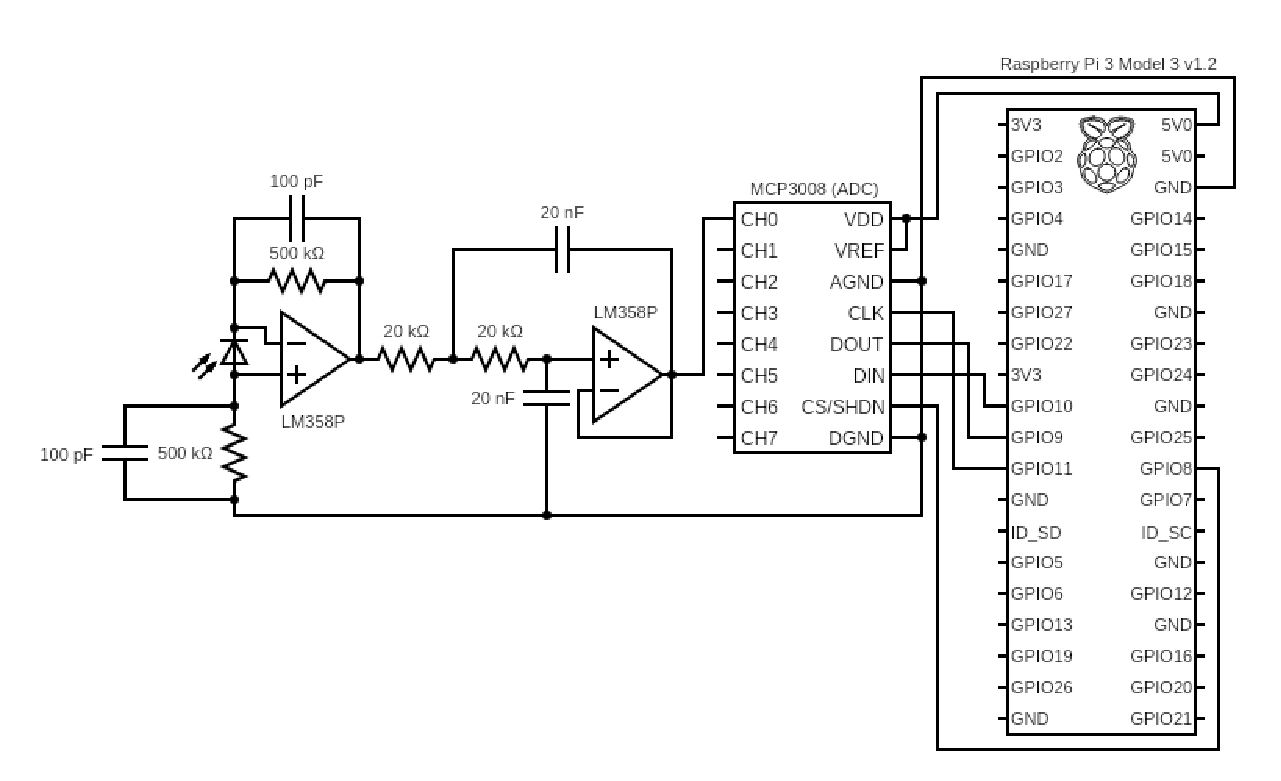
\includegraphics[width=\textwidth]{circuit_diagram.pdf}
	\caption{Circuit diagram for photo-diode reading. Photo-diode in reverse-bias over an op-amp, analog signal then passed through Sallen-Key anti-aliasing filter tuned to 16kHz, then into an analog-to-digital converter (ADC), that’s finally read by the special purpose input (SPI) pins of a Raspberry Pi}
	\label{fig:circuit_diagram}
\end{figure}

\begin{acknowledgments}
We gratefully acknowledge Jude Prezens, Alex Tolotchkoc, Blake Molyneux, Robin Evans, and Bill Moran for their technical advice and generous assistance throughout the project.

The authors are grateful to Deeksha Beniwal, Sebastian Ng, and Craig Ingram for their advice and work in designing the interferometer. 

This research is supported by the Australian Research Council Centre of Excellence for Gravitational Wave Discovery (OzGrav) (project number CE170100004) and the Institute of Physics International Member Grant.

We also acknowledge the ANU PhB program for providing travel funding during the project.


\end{acknowledgments}


\bibliographystyle{myunsrt}
\bibliography{ifoDemoBib}

\end{document}
